% !TEX program = lualatex
% Generated by new_homework.sh — Math 113 Homework 4
\documentclass[11pt]{article}

\usepackage{fontspec}
\usepackage{microtype}
\usepackage{mathtools,amssymb,amsfonts,amsthm,bm}
\usepackage{enumitem}
\usepackage{booktabs,array,xcolor}
\usepackage{geometry,fancyhdr,setspace}
\usepackage{pdfpages}
\usepackage[hidelinks]{hyperref}
\usepackage[nameinlink,noabbrev]{cleveref}

% ---------- Page and paragraph rhythm (matches lecture/solutions templates) ----------
\geometry{margin=1in,headheight=15pt}
\setstretch{1.12}
\setlength{\parindent}{0pt}
\setlength{\parskip}{0.55em plus 0.12em minus 0.08em}
\setlength{\abovedisplayskip}{0.8em plus 0.2em minus 0.1em}
\setlength{\belowdisplayskip}{0.8em plus 0.2em minus 0.1em}
\allowdisplaybreaks[3]
\setlist{leftmargin=*,topsep=0.35em,itemsep=0.15em,parsep=0pt}

% ---------- Metadata ----------
\newcommand{\studentname}{Keshav Ramamurthy}
\newcommand{\coursename}{Math 113}
\newcommand{\courselongname}{Abstract Algebra}
\newcommand{\assignment}{Homework 4}
\newcommand{\term}{Fall 2026}

% ---------- Core notation (same as ~/.config/nvim/textemplate.tex) ----------
\newcommand{\N}{\mathbb{N}}
\newcommand{\Z}{\mathbb{Z}}
\newcommand{\Q}{\mathbb{Q}}
\newcommand{\R}{\mathbb{R}}
\newcommand{\C}{\mathbb{C}}
\newcommand{\F}{\mathbb{F}}
\newcommand{\K}{\mathbb{K}}
\newcommand{\E}{\mathbb{E}}
\newcommand{\Prob}{\mathbb{P}}
\newcommand{\1}{\mathbf{1}}
\newcommand{\eps}{\varepsilon}
\newcommand{\dd}{\,\mathrm{d}}
\newcommand{\abs}[1]{\left\lvert#1\right\rvert}
\newcommand{\norm}[1]{\left\lVert#1\right\rVert}
\newcommand{\ip}[2]{\left\langle#1,#2\right\rangle}
\newcommand{\set}[1]{\left\{#1\right\}}
\newcommand{\ceil}[1]{\left\lceil#1\right\rceil}
\newcommand{\floor}[1]{\left\lfloor#1\right\rfloor}
\newcommand{\given}{\,\middle\vert\,}
\newcommand{\indep}{\perp\!\!\!\perp}
\newcommand{\wh}[1]{\widehat{#1}}
\newcommand{\deriv}[2]{\frac{\mathrm{d}#1}{\mathrm{d}#2}}
\newcommand{\pderiv}[2]{\frac{\partial#1}{\partial#2}}
\newcommand{\lto}{\longrightarrow}
\newcommand{\st}{\text{ such that }}
\DeclareMathOperator{\Aut}{Aut}
\DeclareMathOperator{\End}{End}
\DeclareMathOperator{\Gal}{Gal}
\DeclareMathOperator{\Hom}{Hom}
\DeclareMathOperator{\Ker}{ker}
\DeclareMathOperator{\im}{im}
\DeclareMathOperator{\rank}{rank}
\DeclareMathOperator{\nullity}{nullity}
\DeclareMathOperator{\Span}{span}
\DeclareMathOperator{\tr}{tr}
\DeclareMathOperator{\diag}{diag}
\DeclareMathOperator{\spec}{spec}
\DeclareMathOperator{\ord}{ord}
\DeclareMathOperator{\supp}{supp}
\DeclareMathOperator{\diam}{diam}
\DeclareMathOperator{\Var}{Var}
\DeclareMathOperator{\Cov}{Cov}
\DeclareMathOperator*{\argmin}{arg\,min}
\DeclareMathOperator*{\argmax}{arg\,max}

% ---------- Statement environments ----------
\newtheorem{problem}{Problem}
\newtheorem{theorem}{Theorem}
\newtheorem{lemma}{Lemma}
\newtheorem{proposition}{Proposition}
\newtheorem{corollary}{Corollary}
\theoremstyle{definition}
\newtheorem{definition}{Definition}
\newtheorem{example}{Example}
\newtheorem{remark}{Remark}

% ---------- Solution machinery (matches solutions.tex / textemplate.tex) ----------
\newenvironment{solution}{\begin{proof}[Solution]}{\end{proof}}
\newenvironment{answer}{\begin{proof}[Answer]}{\end{proof}}
\renewcommand{\qedsymbol}{$\square$}
\newcommand{\exercise}[1]{%
  \par\goodbreak\medskip\noindent\textbf{Exercise #1}\par\nopagebreak\smallskip\nopagebreak}
\newcommand{\exref}[1]{\textsf{\textbf{Exercise~#1}}}
\newenvironment{claim}{\par\smallskip\noindent\textit{Claim.}\ }{\par\smallskip}
\newenvironment{idea}{\par\smallskip\noindent\textit{Idea.}\ }{\par\smallskip}
\newenvironment{proofsketch}{\par\smallskip\noindent\textit{Proof sketch.}\ }{\par\smallskip}

% ---------- Header ----------
\pagestyle{fancy}
\fancyhf{}
\fancyhead[L]{\coursename}
\fancyhead[C]{\assignment\ — my solutions}
\fancyhead[R]{\studentname}
\fancyfoot[C]{\thepage}

\begin{document}

% ---------- Title ----------
\begin{center}
  {\Large\sffamily\bfseries \coursename\ -- \courselongname}\par\vspace{3pt}
  {\sffamily \assignment\ — my solutions}\par\vspace{3pt}
  {\small\sffamily \term\quad\textbullet\quad \studentname}
\end{center}
\medskip
\hrule
\bigskip

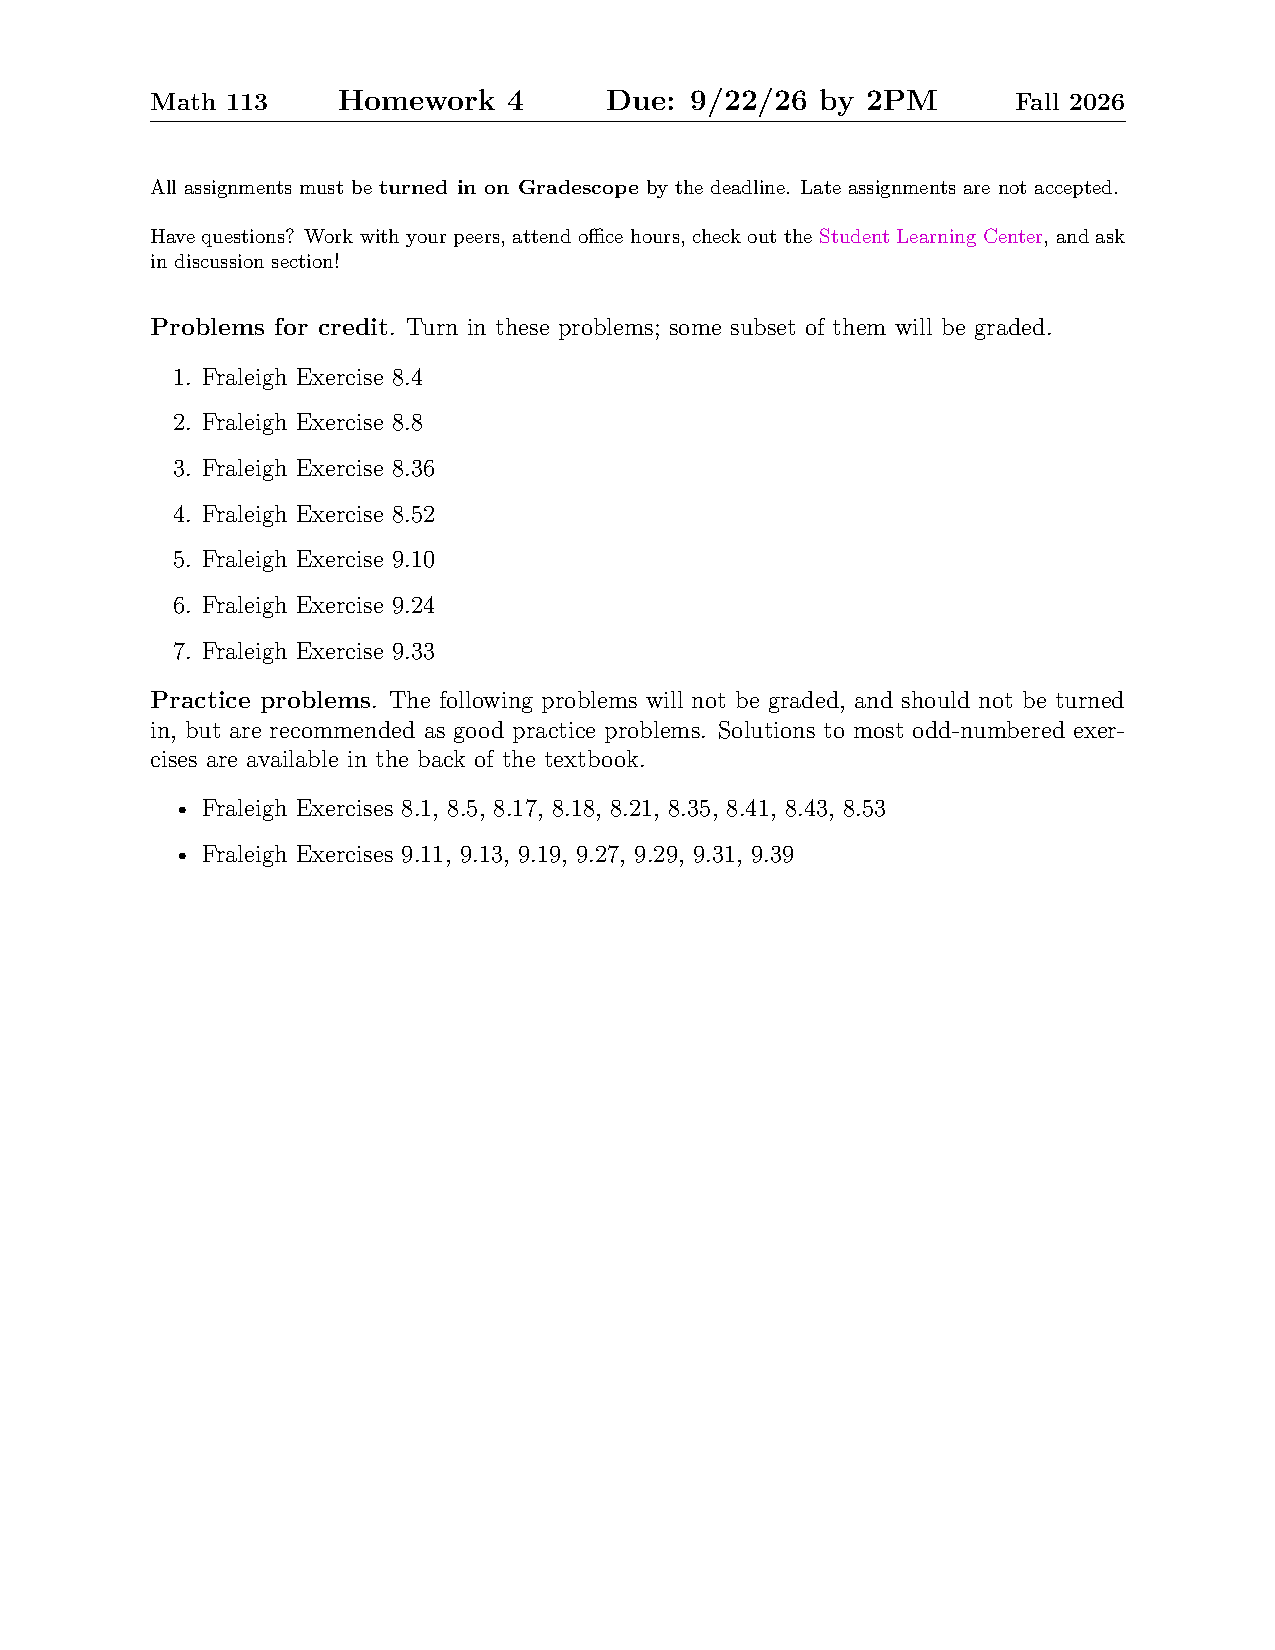
\includepdf[pages=-,pagecommand={\thispagestyle{empty}}]{hw4.pdf}
\clearpage

\section*{Solutions}
\subsubsection*{Problem 1 (Fraleigh Exercise 8.4)}
\begin{solution}
    First write $\sigma$ and $\tau$ as disjoint cycles:
    $$\sigma = (1,3,4,5,6,2), \qquad \tau = (1,2,4,3)(5,6).$$
    \par Squaring the $6$-cycle moves two steps at a time, so $\sigma^2 = (1,4,6)(2,3,5)$.
    \par Inverting reverses each cycle, so $\sigma^{-2} = (1,6,4)(2,5,3)$.
    \par Now $\sigma^{-2}\tau$ means apply $\tau$ first, then $\sigma^{-2}$. Tracing each element:
    $$1 \to 2 \to 5, \quad 5 \to 6 \to 4, \quad 4 \to 3 \to 2, \quad 2 \to 4 \to 1,$$
    so we get $(1,5,4,2)$.
    \par And $3 \to 1 \to 6$, $6 \to 5 \to 3$ gives $(3,6)$.
    \par Thus
    $$\sigma^{-2}\tau = (1,5,4,2)(3,6).$$
% Write your proof, calculation, or argument here.
\end{solution}
\subsubsection*{Problem 2 (Fraleigh Exercise 8.8)}
\begin{solution}
    $\sigma$ is a $6$-cycle, so it returns to the identity after exactly $6$ applications.
    That is, $\abs{\sigma} = 6$. Hence the exponent reduces modulo $6$: $100 = 96 + 4$, so
    $$\sigma^{100} = \sigma^4.$$
    \par From Problem 1, $\sigma^2 = (1,4,6)(2,3,5)$, so squaring once more gives
    $\sigma^4 = (1,6,4)(2,5,3)$.
% Write your proof, calculation, or argument here.
\end{solution}
\subsubsection*{Problem 3 (Fraleigh Exercise 8.36)}
\begin{solution}
    $S_3$ works. It's nonabelian since
    $$(1,2)(1,3) = (1,3,2) \quad \text{but} \quad (1,3)(1,2) = (1,2,3).$$
    \par Now take any proper subgroup $H$ of $S_3$. The identity has order $1$, the three
    transpositions have order $2$, and the two $3$-cycles have order $3$. So $H$ can't have
    order $5$ (that would need an element of order $5$), and it can't have order $4$ either:
    its three nonidentity elements would all have to be transpositions, but any two distinct
    transpositions in $S_3$ multiply to a $3$-cycle, which would have to be in $H$ too. So
    $H$ has order $1$, $2$, or $3$.
    \par If $\abs{H} = 2$, then $H = \{e, g\}$ with $g^2 = e$.
    \par If $\abs{H} = 3$, then $H = \{e, g, g^2\}$.
    \par In either case every element is a power of a single $g$, so any two elements are
    powers $g^i, g^j$, which commute. Thus $H$ is abelian.
% Write your proof, calculation, or argument here.
\end{solution}
\subsubsection*{Problem 4 (Fraleigh Exercise 8.52)}
\begin{solution}
    Let $H = \set{\rho_a \given a \in G}$.
    \par Each $\rho_a$ is a permutation of $G$. If $\rho_a(x) = \rho_a(y)$, then $xa = ya$, and
    multiplying both sides by $a^{-1}$ on the right gives $x = y$, so it's one-to-one.
    \par It's onto too, since any $y$ is hit by $y = \rho_a(ya^{-1})$.
    \par Composing two of them:
    $$(\rho_a \circ \rho_b)(x) = \rho_a(xb) = (xb)a = x(ba) = \rho_{ba}(x),$$
    so $\rho_a \circ \rho_b = \rho_{ba}$.
    \par So the set is closed under composition.
    \par We have that $\rho_e$ is the identity, and $\rho_{a^{-1}}$
    is the inverse of $\rho_a$ since $\rho_a \circ \rho_{a^{-1}} = \rho_e$. Thus $H \le S_G$.
    \par Since composing $\rho_a$ and $\rho_b$ gives $\rho_{ba}$, we fix the order of the
    subscripts by using $a \to \rho_{a^{-1}}$ instead of $a \to \rho_a$. Define
    $\phi : G \to H$ by $\phi(a) = \rho_{a^{-1}}$. Then
    $$\phi(ab) = \rho_{(ab)^{-1}} = \rho_{b^{-1}a^{-1}} = \rho_{a^{-1}} \circ \rho_{b^{-1}} = \phi(a)\phi(b).$$
    \par Finally, $\phi$ is onto by definition, and it's one-to-one since $\phi(a) = \phi(b)$
    means $\rho_{a^{-1}} = \rho_{b^{-1}}$, and evaluating at $e$ gives $a^{-1} = b^{-1}$, so
    $a = b$. So $\phi$ is an isomorphism, and $G \cong H$.
% Write your proof, calculation, or argument here.
\end{solution}
\subsubsection*{Problem 5 (Fraleigh Exercise 9.10)}
\begin{solution}
    We have 
    $$\sigma = \begin{pmatrix}
    1 & 2 & 3 & 4 & 5 & 6 & 7 & 8\\
    8 & 2 & 6 & 3 & 7 & 4 & 5 & 1
    \end{pmatrix}.$$
    \par $1 \to 8 \to 1$ gives $(1,8)$.
    \par $2$ is fixed.
    \par $3 \to 6 \to 4 \to 3$ gives $(3,6,4)$.
    \par And $5 \to 7 \to 5$ gives $(5,7)$.
    \par So
    $$\sigma = (1,8)(3,6,4)(5,7).$$
    \par Finally, $(3,6,4) = (3,4)(3,6)$, so
    $$\sigma = (1,8)(3,4)(3,6)(5,7).$$
% Write your proof, calculation, or argument here.
\end{solution}
\subsubsection*{Problem 6 (Fraleigh Exercise 9.24)}
\begin{solution}
    \par The identity is even, being the empty product. The $3$-cycles are even as well,
    since $(1,2,3) = (1,3)(1,2)$ and $(1,3,2) = (1,2)(1,3)$. The $\mu$'s are transpositions,
    hence odd.
    \par Thus
    $$A_3 = \{\rho_0, \rho_1, \rho_2\},$$
    with multiplication table
    \begin{center}
    \begin{tabular}{c|ccc}
             & $\rho_0$ & $\rho_1$ & $\rho_2$ \\ \hline
    $\rho_0$ & $\rho_0$ & $\rho_1$ & $\rho_2$ \\
    $\rho_1$ & $\rho_1$ & $\rho_2$ & $\rho_0$ \\
    $\rho_2$ & $\rho_2$ & $\rho_0$ & $\rho_1$
    \end{tabular}
    \end{center}
% Write your proof, calculation, or argument here.
\end{solution}
\subsubsection*{Problem 7 (Fraleigh Exercise 9.33)}
\begin{solution}
    Take any odd $\tau$. We need $\tau = \sigma\mu$ for some $\mu \in A_n$, so solve for
    $\mu$: $\mu = \sigma^{-1}\tau$. Since $\sigma^{-1}$ is also odd, $\sigma^{-1}\tau$ is
    even, so $\mu \in A_n$.
    \par Then
    $$\sigma\mu = \sigma(\sigma^{-1}\tau) = \tau.$$
    so we are done.
% Write your proof, calculation, or argument here.
\end{solution}

\end{document}
